\chapter{Project Plan}

\section{Meetings}
Our goals were outlined by weekly meetings. We regularly met with Jacob Graff, our advisor throughout the development of Extend.
Jacob served as a sounding board whenever Extend's fundamental design philosophy was debated, and as a guide as we determined whether we were on track. We used any leftover time on those days to set goals for the upcoming week and pair program if time permitted.
\newline \newline
Our team also met weekly on Fridays to further discuss the progression of Extend. In the first half of the semester, the discussions were primarily philosophical, as decisions had to be made about the language grammar and behavior of certain Extend artifacts prior to development. In the second half, time was devoted to ironing out the development timeline, discussing bugs, and making compiler implementation decisions.

\section{Development Workflow}
  \begin{center}
  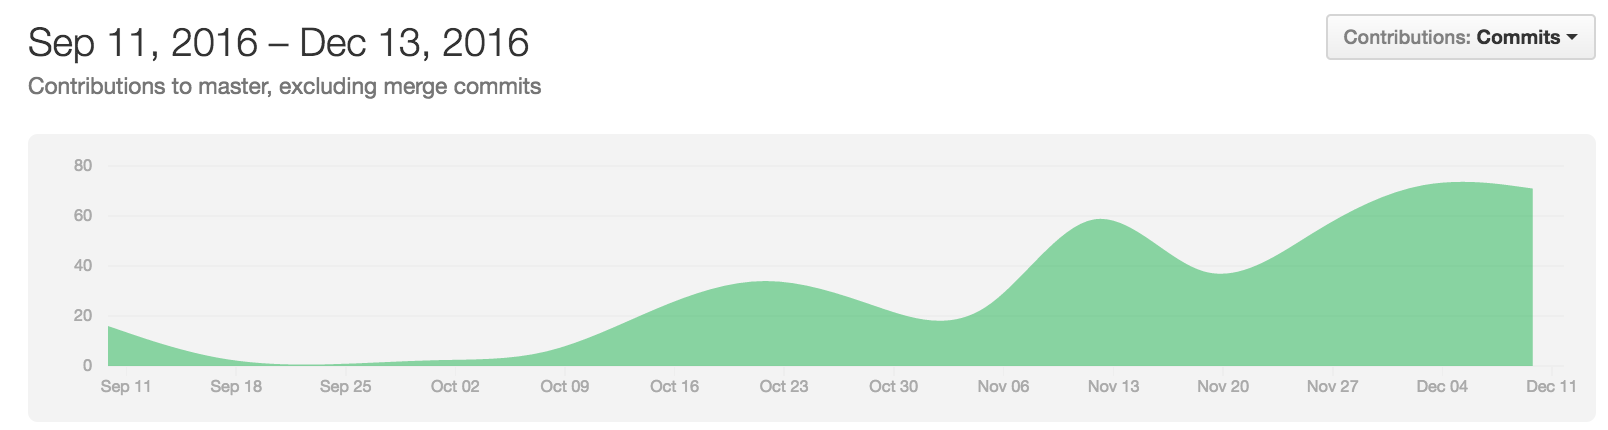
\includegraphics[width=.9\textwidth]{img/extend_git_graph.png}
  \end{center}

  \subsection{Github \& Travis CI}
  Our development and documentation were all done entirely through version control to maximize independent productivity.
  New features were introduced to the master branch through pull requests, and the team used this as a platform to peer review code to maximize code quality before such features entered production.

  \medskip \noindent
  An important aspect of development for us was continuous integration. Each pull request we made triggered a Travis build, which kept us informed regarding unexpected hiccups that sometimes arose during development. Travis CI ensured that new features were implemented with protecting the code base in mind, and provided quick visibility as to whether a new feature would break the existing build. Any changeset to the master branch must:

  \begin{enumerate}
    \item Pass Travis CI.
    \item Be approved by another member of the team.
    \item Be up to date with the master branch.
  \end{enumerate}
  
\subsection{Style Guide}
  None of the team members had any prior experience with Ocaml. Fundamentally we were developing a certain style in the process of creating the project. A few style choices were clear soon after starting to develop in Ocaml:
  \begin{itemize}
  \item Avoid deep nesting of functions
  \item Instead build better abstraction and reuse functions
  \item Use \textbf{let ... in} instead of \textbf{and}. While this creates a lot of closures, it helped us to develop quicker by not needing to restructure code for changes
  \item Use underscore for values you won't use any further. Llvm code generation inherently creates a lot of values where the return value is of no use. Therefore mark those return values with an underscore, since it hides the warning. 
  \item Indent with spaces, not tabs. Indent by 2 for each level of nesting.
  \item Make intentions clear by naming return values, not by naming LLVM indermediate values.
  \end{itemize}
These few rules helped us to control our code very well.\newline
Further we were developing our runtime in C. We applied the following style rules:
  \begin{itemize}
  \item Indent with tabs.
  \item Stick to C99.
  \item Use \textbf{value\_p} for user facing functions.
  \item Make sure to exit gracefully.
  \end{itemize}

\section{Language Evolution}
Looking back at our original proposal, the language we delivered ended up surprisingly close. The biggest change was to allow strings and ranges as value types, which made the language immeasurably better. Initially, we wanted to only have Numbers; but allowing cells to contain ranges (composite values) and not just primitive values makes it a much more useful language. Otherwise, the syntax and semantics are very close to what was in our original proposal.

Our initial plan was to precalculate the dependencies among cells as best as possible at compile time and generate code accordingly. However, it quickly became clear that the language was better with runtime-determined cell dependencies and we therefore had to give up on a precomputed graph. We didn't have time in this class to implement an explicit stack as opposed to using recursion, but this could be overcome if it had to be.

Another fairly minor change was to eliminate the dimension signature for functions. As we played around with the language in the interpreter, it became clear that we weren't using them and it wasn't obvious why we would; they were dropped as a result.


  \subsection{The Interpreter}
  In our efforts to maximize our effectiveness when building the compiler, we additionally built a working interpreter to test the language semantics and run example Extend programs. This helped us determine language decisions at an earlier stage in the process, and helped us benchmark the success of our compiler by comparing the number of testcases passed by both.

\section{Team Member Responsibilities}

\begin{tabular}{ | l | l | l |}\hline
  Team Member  & Responsibilities      & GitHub Profile\\ \hline
  Jared Samet & design philosophy, semantic transformations, code generation  & \underline{\href{https://github.com/oracleofnj}{oracleofnj}}\\
  Nigel Schuster & development protocol, code generation, scripting  & \underline{\href{https://github.com/Neitsch}{Neitsch}}\\
  Ishaan Kolluri & initial LRM, Final Report, regression tests, stdlib functions, scripting & \underline{\href{https://github.com/ishaankolluri}{ishaankolluri}}\\
  Kevin Ye & initial scanner, regression tests, stdlib functions & \underline{\href{https://github.com/kevinye1}{kevinye1}}\\ \hline
\end{tabular}
